\documentclass{beamer}
\usetheme{Madrid}

\usepackage{amsmath, amssymb, amsthm}
\usepackage{graphicx}
\usepackage{listings}
\usepackage{gensymb}
\usepackage[utf8]{inputenc}
\usepackage{hyperref}
\usepackage{gvv}
\usepackage{tikz}
\lstset{
  language=Python,
  basicstyle=\ttfamily\small,
  keywordstyle=\color{blue},
  stringstyle=\color{orange},
  numbers=left,
  numberstyle=\tiny\color{gray},
  breaklines=true,
  showstringspaces=false
}
\usetikzlibrary{decorations.pathmorphing}

\title{Question-2.4.16}
\author{EE25BTECH11022 - sankeerthan}
\date{}
\begin{document}

\frame{\titlepage}

\begin{frame}
\frametitle{Question}
show that the line through the points \brak{1,-1,2} , \brak{3,4,-2} is perpendicular to the line through the  points  \brak{0,3,2} and \brak{3,5,6}
\end{frame}

\begin{frame}
\frametitle{Solution}\begin{align}
let \Vec{A} =\brak{1,-1,2},\Vec{B} =\brak{3,4,-2},\Vec{C} =\brak{0,3,2},\Vec{D} =\brak{3,5,6}
\end{align}
Direction vector of line joining points $\Vec{A}$ and $\Vec{B}$ is
\begin{align}
    \Vec{B}-\Vec{A} &= \myvec{3-1 \\ 4-(-1) \\ -2-2}\\
    &= \myvec{2 \\ 5 \\-4}\\
\end{align}
Direction vector of line joining points $\Vec{C}$ and $\Vec{D}$ is
\end{frame}

\begin{frame}
\frametitle{Solution}
\begin{align}
    \Vec{C}-\Vec{D} &= \myvec{3-0 \\ 5-3 \\ 6-2}\\
    &= \myvec{3 \\ 2 \\4}\\
\myvec{\vec{B}-\vec{A}}^\top\myvec{\vec{D}-\vec{C}} &= \myvec{2 \ \ 5 \ \ -4}\myvec{3 \\ 2 \\4}\\
 &= 2\brak{3}+5\brak{2}+\brak{-4}\brak{4}\\
 &=6+10-16 =0\\
 \myvec{\vec{B}-\vec{A}}^\top\myvec{\vec{D}-\vec{C}} = 0
\end{align}
Therefore, the lines joining points $\Vec{A}$,$\Vec{B}$ and $\Vec{C}$,$\Vec{D}$ are perpendicular 

\end{frame}

\begin{frame}
\frametitle{graph}
\begin{figure}
    \centering
    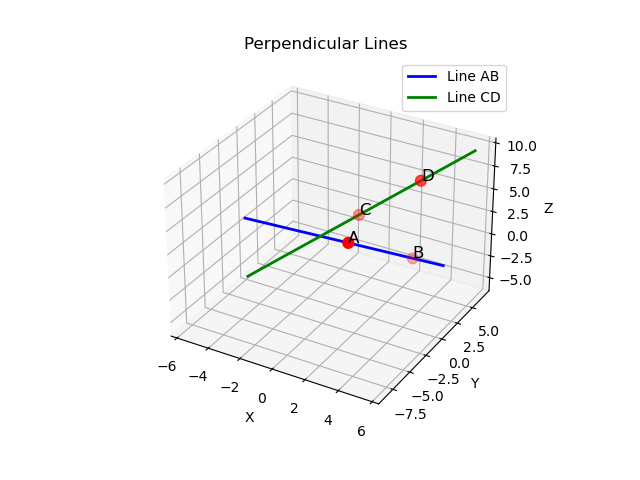
\includegraphics[width=\linewidth]{figs/points.png}
    \caption{}
\end{figure}
\end{frame}

\begin{frame}[fragile]
\frametitle{C-Code}
\begin{lstlisting}[language=C]
// code.c
#define NUM_POINTS 4

void get_points(double *arr) {
    double points[NUM_POINTS][3] = {
        {1, -1, 2},
        {3,  4, -2},
        {0,  3,  2},
        {3,  5,  6}
    };
    for (int i = 0; i < NUM_POINTS; ++i)
        for (int j = 0; j < 3; ++j)
            arr[i*3 + j] = points[i][j];
}

 \end{lstlisting}
\end{frame}

\begin{frame}[fragile]
\frametitle{C-Code}
\begin{lstlisting}[language=C]

void get_dir_vectors(double *v1, double *v2) {
    // v1: AB; v2: CD
    v1[0] = 3 - 1;
    v1[1] = 4 - (-1);
    v1[2] = -2 - 2;
    v2[0] = 3 - 0;
    v2[1] = 5 - 3;
    v2[2] = 6 - 2;
}

int check_perpendicular() {
    double v1[3], v2[3];
    get_dir_vectors(v1, v2);
    double dot = v1[0]*v2[0] + v1[1]*v2[1] + v1[2]*v2[2];
    return dot == 0 ? 1 : 0;
}


 \end{lstlisting}
\end{frame}
\begin{frame}[fragile]
\frametitle{Python-Code}
\begin{lstlisting}
# Code by GVV Sharma
# Modified for Problem Solution
# Released under GNU GPL
# Calculating area enclosed between curves
# call.py
import ctypes

lib = ctypes.CDLL('./libcode.so')

# Perpendicularity check from C
result = lib.check_perpendicular()

\end{lstlisting}
\end{frame}

\begin{frame}[fragile]
\frametitle{Python-Code}
\begin{lstlisting}
print("The lines are perpendicular." if result else "The lines are not perpendicular.")

# Extract and print the points
arr = (ctypes.c_double * 12)()
lib.get_points(arr)
for i in range(4):
    print(f"Point {chr(65 + i)}: ({arr[i*3]}, {arr[i*3 + 1]}, {arr[i*3 + 2]})")

\end{lstlisting}
\end{frame}

\begin{frame}[fragile]
\frametitle{Python-Code}
\begin{lstlisting}
import ctypes
import numpy as np
import matplotlib.pyplot as plt

# Load .so and extract points
lib = ctypes.CDLL('./libcode.so')
arr = (ctypes.c_double * 12)()
lib.get_points(arr)
pts = np.array(arr).reshape((4,3))
A, B, C, D = pts

fig = plt.figure()
ax = fig.add_subplot(111, projection='3d')


\end{lstlisting}
\end{frame}

\begin{frame}[fragile]
\frametitle{Python-Code}
\begin{lstlisting}
ax.plot([A[0], B[0]], [A[1], B[1]], [A[2], B[2]], color='blue', label='Line AB')
ax.plot([C[0], D[0]], [C[1], D[1]], [C[2], D[2]], color='green', label='Line CD')

# Plot and annotate points
ax.scatter(pts[:,0], pts[:,1], pts[:,2], color='red', s=70)
for i, label in enumerate(['A','B','C','D']):
    ax.text(pts[i,0], pts[i,1], pts[i,2], label, size=12)

ax.set_xlabel('X')
ax.set_ylabel('Y')
ax.set_zlabel('Z')
ax.set_title('3D Plot of Two Perpendicular Lines')
ax.legend()
plt.show()

\end{lstlisting}
\end{frame}

\end{document}